\chapter{Força entre corrents}
\begin{resum}
Aquest informe presenta els resultats de l'estudi de la força exercida entre dos corrents paral·lels pels quals hi circula la mateixa intensitat. Concretament, s'ha provat experimentalment la dependència lineal entre la força i el quadrat de la intensitat i entre la força i l'invers de la distància entre els fils.

A més, s'ha trobat experimentalment el valor de la constant \( \mu_0 \) a partir de la llei de Biot-Savart, \( \mu_0 = \data{1.25}{0.04e-6}{N.A^{-2}} \) i \( \mu_0 = \data{3.0}{0.4d-6}{N.A^{-2}} \). El primer valor és consistent amb el tabulat, mentre que el segon només n'és de l'ordre. 

Finalment, s'ha mesurat la component radial del camp magnètic terrestre, obtenint un valor de \( B = \data{1.59}{0.18d-5}{T} \) de l'ordre del que descriuen altres articles.
\end{resum}

\begin{multicols}{2}
	\section{Introducció i Objectius}
	L'objectiu principal d'aquesta pràctica és la comprovació experimental de la llei de Biot-Savart en el cas de dos fils paral·lels. S'ha calculat la força que s'exerceixen dos fils paral·lels pels quals hi circula la mateixa intensitat.

	Més concretament, s'han avaluat experimentalment les correlacions entre la força entre els corrents i el quadrat de la intensitat que hi circula, i també entre la força i l'invers de la distància a què es troben.

	A més, s'ha determinat experimentalment la constant $\mu_0$ i el valor de la component radial del camp magnètic terrestre.

	A partir de la llei d'Àmpere, es pot deduir que la força que s'exerceixen dos fils amb les característiques mencionades anteriorment és 

	\begin{equation}
		\mathbf{F}=\frac{\mu_0I^2L}{2\pi r} \hat{ \mathbf{r} } 
	\end{equation}
	on $I$ és la intensitat que hi circula, $L$ la longitud dels dos fils i $r$ la separació entre ells.

	També, si existeix un camp $B$ constant al llarg de tot el fil, la força que sent aquest és

	\begin{equation}
		F=BLI
	\end{equation}

	\section{Mètode experimental}
	Totes les mesures s'han pres en una balança de corrents. La Figura 1 mostra un esquema del dispositiu, amb els elements principals.
	\begin{figure}
		\centering
		% 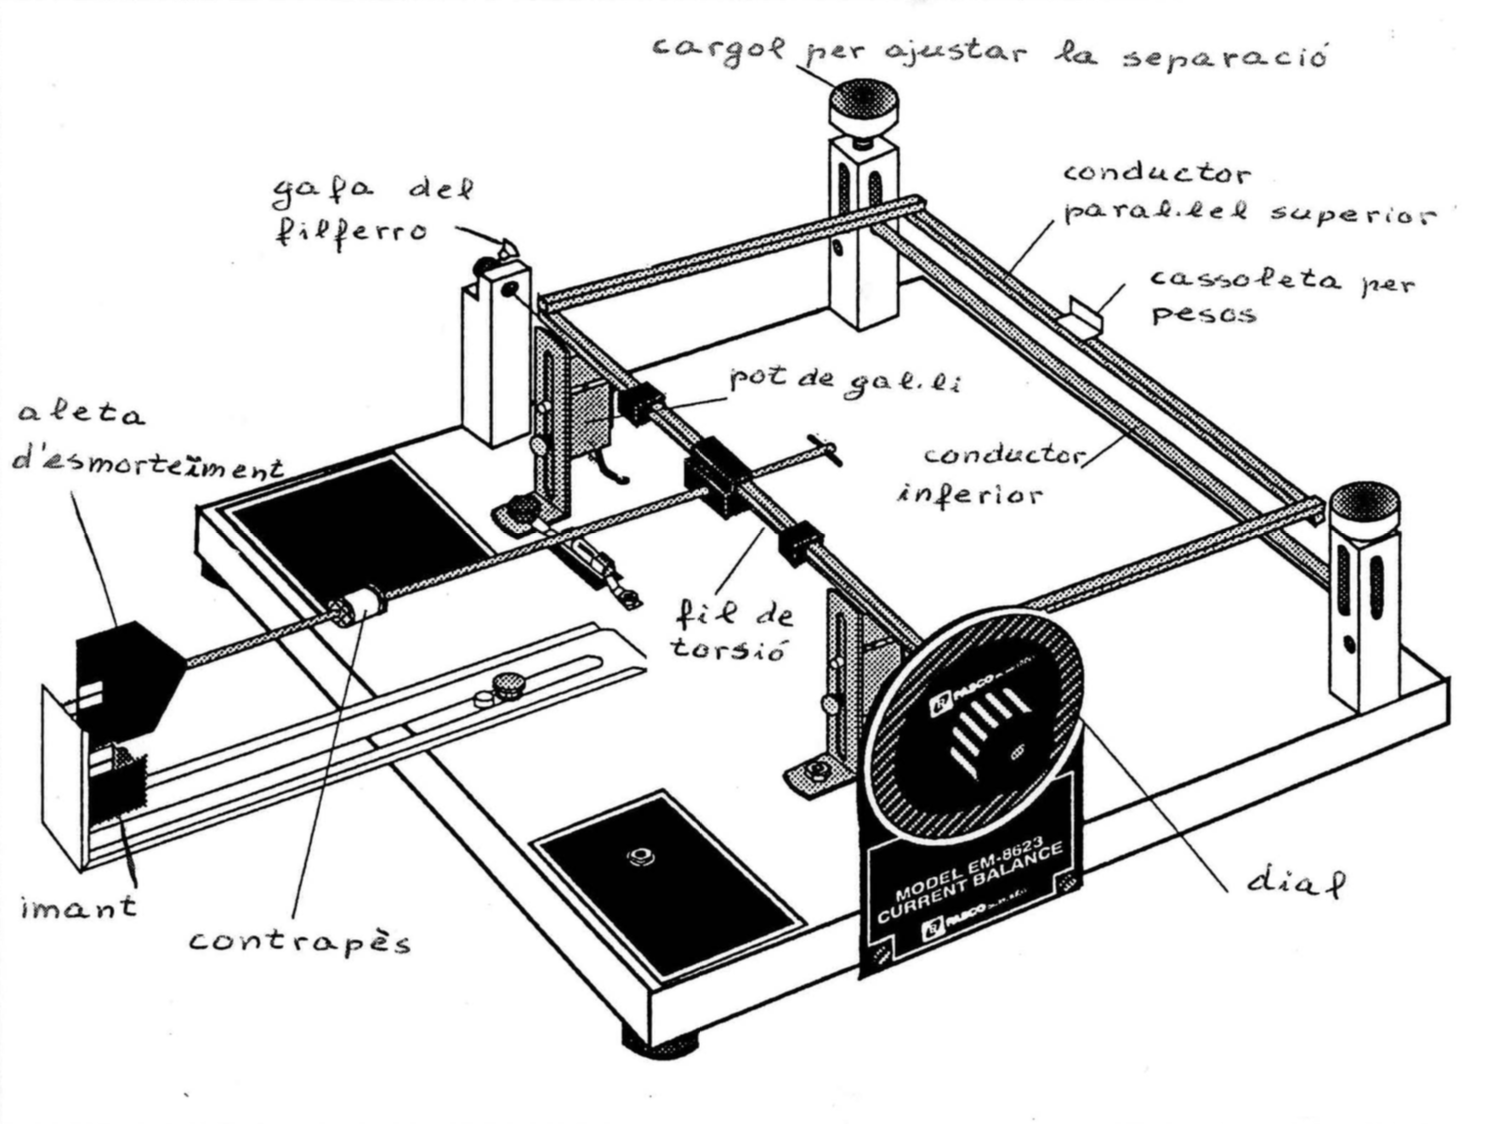
\includegraphics[scale=0.5]{Fig1.png}
		\caption{Esquema de la balança de corrents amb els principals elements}
	\end{figure}

	La balança disposa de dos maneres de determinar la força entre els corrents. Per una banda, disposa d'una cassoleta de pesos on col·locar diferents masses. Sabent que, en el moment que la balança es troba equilibrada, la força gravitatòria sobre la massa és igual a la força entre els corrents es pot determinar aquesta última. Per l'altra banda, la balança també disposa d'un dial i un fil de torsió que poden contrarrestar la força entre els corrents. Sabent que la relació entre els graus que rota el dial i la força que fa és lineal, i coneixent la constant de proporcionalitat es pot determinar també la força entre els corrents.

	Creiem necessari comentar que els corrents s'han disposat en direcció nord-sud terrestre per tal que el camp magnètic de la Terra no influís en els nostres resultats.

	Cal també comentar que el valor que s'ha pres com a acceleració de la gravetat és $9.80665 \si{m/s^2}$ sense incertesa, ja que s'ha considerat que és menyspreable enfront a la resta d'incerteses que puguem tenir. S'han pres també sense incertesa els valors de les masses proporcionades al laboratori.

	\subsection{Força vs. Intensitat}

	Per aquesta part de la pràctica s'ha mesurat la intensitat necessària per compensar la força gravitatòria exercida sobre el cable superior per masses de $5,\ 10,\ 15,\ 20$ i $25\si{mg}$. Posteriorment s'ha aplicat una regressió lineal entre la força i el quadrat de la intensitat per comprovar-ne la correlació predita per l'expressió 2.

	\subsection{Força vs. Distància}
	En aquesta part, s'ha fixat una intensitat i s'ha anat variant la distància entre els cables amb els cargols disposats amb aquest fi. Per cada distància desitjada s'ha determinat la força entre els corrents a partir del dial i el fil de torsió. A les dades preses se'ls hi ha aplicat una regressió lineal entre la força i l'invers de la distància de separació per comprovar la correlació predita per l'expressió 2. A partir del pendent obtingut en la regressió i l'expressió 2 s'ha determinat experimentalment la constant $\mu_0$.
	\subsection{Camp Magnètic Terrestre}
	Per aquesta part de l'experiència %Arnau I lof u
	s'han orientat els corrents en direcció est-oest per tal que influís la component radial del camp magnètic terrestre. Per la disposició de la balança i el fet que la força que un camp magnètic exerceix sobre un corrent és perpendicular al pla que defineixen no es pot determinar la component horitzontal del camp magnètic terrestre.

	Posteriorment, s'ha fet circular una intensitat fixa només pel fil superior i s'ha determinat la força que patia a través del dial i el fil de torsió. El camp magnètic s'ha determinat a partir de l'expressió 3. 
\end{multicols}
